
% make sure pub/subs are consistent

% Paper guidelines require all content other than figures in a single tex file.
% Unused packages should be removed (not just commented out)
% Detailed instructions are at: http://tab.computer.org/tcde/bull_author.html


% Use of dvipdfm makes the figures disappear
%\documentclass[11pt,dvipdfm]{article}
%\documentclass[11pt]{article}

%\usepackage[utf8]{inputenc}
%\usepackage{deauthor,times}
%\usepackage[final]{graphicx}
%\usepackage{array}
%\usepackage{subfig}
%\usepackage{wrapfig}
%\usepackage[table]{xcolor}
%\usepackage{tcolorbox}
%\usepackage{amssymb}

%\graphicspath{ {./figs/} }



%%%
\hyphenation{finally}

\begin{document}


\title{Extending the Publish/Subscribe Abstraction for High-Performance I/O and Data Management at Extreme Scale}

\author{
Jeremy Logan$\dagger$,
Mark Ainsworth$\S$,
Chuck Atkins$\ddagger$,
Jieyang Chen$\dagger$,
Jong Choi$\dagger$,
Junmin Gu$\star$, \\
James Kress$\dagger$, 
Greg Eisenhauer$\circledcirc$,
Berk Geveci$\ddagger$,
William Godoy$\dagger$, 
Mark Kim$\dagger$, \\
Tahsin Kurc$\dagger$,
Qing Liu$\cup$, 
Kshitij Mehta$\dagger$, 
George Ostrouchov$\dagger$, 
Norbert Podhorzski$\dagger$, \\
David Pugmire$\dagger$, 
Eric Suchyta$\dagger$, 
Nicolas Thompson$\dagger$, 
Ozan Tugluk$\S$,
Lipeng Wan$\dagger$, \\
Ruonan Wang$\dagger$, 
Ben Whitney$\dagger$,
Matthew Wolf$\dagger$,
Kesheng Wu$\star$,
and Scott Klasky$\dagger$
}
\maketitle

\begin{center}
   {$\S$ \hspace{0em} Brown University, Providence, RI, USA}
   
   {$\circledcirc$ \hspace{0em} Georgia Institute of Technology, Atlanta, GA, USA}
   
   {$\ddagger$ \hspace{0em} Kitware, Inc., Clifton Park, NY, USA}
   
   {$\star$ Lawrence Berkeley National Laboratory, Berkeley, CA, USA}
   
   {$\cup$ \hspace{0em} New Jersey Institute of Technology, Newark, New Jersey, USA}
   
   {$\dagger$ Oak Ridge National Laboratory, Oak Ridge, TN, USA}
\end{center}
\vspace{1.0em}



\begin{abstract}
The Adaptable I/O System (ADIOS) represents the culmination of substantial investment in Scientific
Data Management, and it has demonstrated success for several important extreme-scale science cases.
However, looking towards the exascale and beyond, we see the development of yet more stringent data management
requirements that require new abstractions. Therefore, there is an opportunity to attempt to connect the
traditional realms of HPC I/O optimization with the Database / Data Management community. In this
paper, we offer some specific examples from our ongoing work in managing data structures, services, and
performance at the extreme scale for scientific computing. 
%We evaluate these examples using Cori at the National Energy Research Scientific Computing Center (NERSC) and Summit at the Oak Ridge Leadership Computing Facility (OLCF). 
Using the publish/subscribe model afforded
by ADIOS, we demonstrate a set of services that connect data format, metadata, queries, data reduction,
and high-performance delivery. 
The resulting publish/subscribe framework facilitates connection to on-line workflow systems to enable the dynamic capabilities that will be required for exascale science.

\let\thefootnote\relax\footnotetext{Notice:  This manuscript has been authored by UT-Battelle, LLC, under contract DE-AC05-00OR22725 with the US Department of Energy (DOE). The US government retains and the publisher, by accepting the article for publication, acknowledges that the US government retains a nonexclusive, paid-up, irrevocable, worldwide license to publish or reproduce the published form of this manuscript, or allow others to do so, for US government purposes. DOE will provide public access to these results of federally sponsored research in accordance with the DOE Public Access Plan (http://energy.gov/downloads/doe-public-access-plan).}

% \makeatletter
% \footnote{Notice:  This manuscript has been authored by UT-Battelle, LLC, under contract DE-AC05-00OR22725 with the US Department of Energy (DOE). The US government retains and the publisher, by accepting the article for publication, acknowledges that the US government retains a nonexclusive, paid-up, irrevocable, worldwide license to publish or reproduce the published form of this manuscript, or allow others to do so, for US government purposes. DOE will provide public access to these results of federally sponsored research in accordance with the DOE Public Access Plan (http://energy.gov/downloads/doe-public-access-plan).}
% \makeatother
\end{abstract}



\section{Introduction 
%\textcolor{red}{- 1.5 Pgs}
}


While exascale systems are poised to arrive at Leadership Computing Facilities and provide never-before-seen capacity for sheer computational ability, a new generation of science applications are evolving that will leverage these systems to push the boundaries of science. Changes in the way that science applications are built and used are creating new challenges to the Applied Math and Computer Science communities which must be met in order to fully utilize these new HPC systems. 
There are several important categories of changes that are occurring in this context.
First, as scientists seek to extend the impact of simulation, there is an increased need to couple together multiple separate applications. One variant of this is multi-physics code coupling, where several established simulation codes are made to share data in order to work together to accomplish a larger task. This type of coupling, known as \textit{strong coupling}, typically involves applications that are interdependent and rely on data from each other in order to continue. This contrasts with \textit{weak (in situ) coupling}, where data producers do not have any dependence on consumers and can continue working unfettered regardless of the progress or presence of subsequent workflow components. Weak coupling capabilities are increasingly in demand as a technique for applying machine learning/AI techniques to understand the data as it is being produced.
Another increasingly prevalent technique, seen in areas such as molecular dynamics and seismology, involves the use of large ensembles of individual simulations, along with the subsequent statistical analysis of the large set of resulting data.
Finally, federating large-scale experimental and observational facilities with exascale simulation environments to provide real-time analysis and steering of ongoing measurements will be essential for leveraging these facilities to best benefit science.
The need to extend the existing high performance I/O and data management capabilities to support these new categories is currently a major driver of our work. 
\begin{wrapfigure}{o}{3.2in}
\vspace{-10pt}
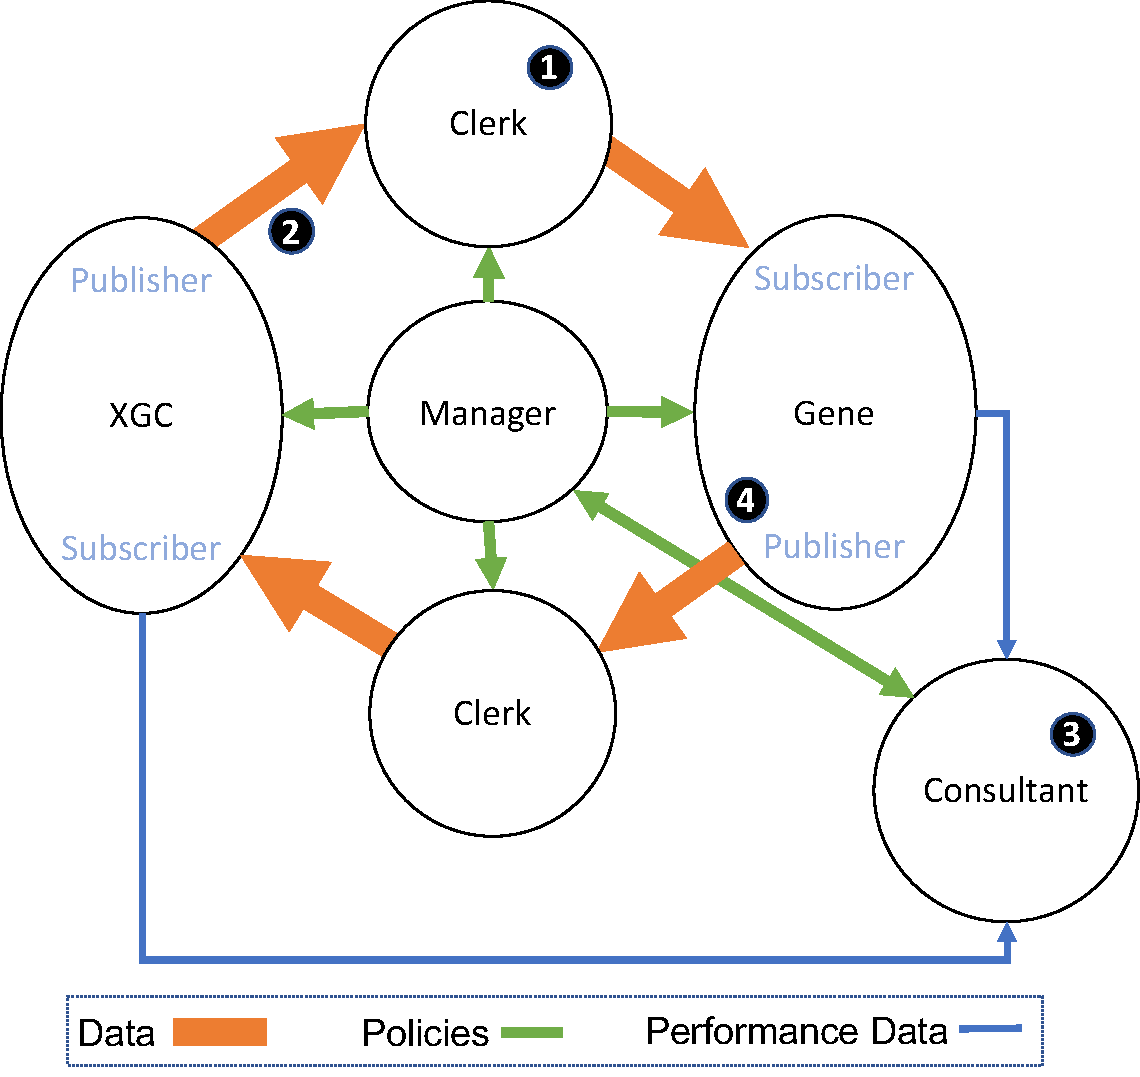
\includegraphics[width=3.2in]{figs/capabilities.pdf}
\caption{A logical view of a code coupling example involving two fusion codes, XGC1 and Gene, which focus on different regions of a reactor. Enhanced capabilities include 1) Data compression within a publish/subscribe stream, 2) Strong coupling provided by a pair of pub/sub streams, 3) Performance understanding provided by a Consultant capable of advising a Manager, and 4) Enhanced metadata.}
\label{fig:capabilities}
\vspace{-.1in}
\end{wrapfigure}

The Adaptable I/O System (ADIOS)~\cite{HelloAdios} has been developed to offer high-performance I/O, staging, data reduction, and data management capabilities to applications through a simple publish/subscribe oriented API. 
%As we have continued to develop this range of capabilities, it has become more challenging for users to comprehend the available options and to determine which are applicable to a particular application. 
In \S\ref{sec:models} we present several of the underlying models upon which our tools are based. First, we explore some useful extensions to the publish/subscribe pattern, and describe how ADIOS is being used to support such an approach to data management. Then we introduce the Streaming Structure of Parallel Arrays (SSOPA) model that describes the underlying approach used by ADIOS to manage distributed self-describing data.

%\todo[inline]{Kshitij, please edit the following to be more specific to ADIOS.}

%wrapfig {o} is outside (away from spine)



To address the changing set of usage patterns on leadership computing platforms, we present a set of capabilities that are needed to facilitate effective use of these machines by current and emerging science use cases, and in particular, how we are incorporating these capabilities into the ADIOS ecosystem. First, as I/O and storage capacity is generally failing to keep pace with advances in computational capabilities, data compression and reduction capabilities are an increasingly critical requirement for exascale. We have incorporated a variety of compression capabilities into ADIOS, and ongoing work with MGARD~\cite{ainsworth2018multilevel} offers a novel data refactoring capability that will allow different levels of data resolution to be provided according to the user's intentions. Next, we have developed a variety of data staging services to address different runtime needs of applications and \textit{in situ} workflow components. Runtime performance understanding is critical for maintaining high utilization levels for exascale workflows, and we discuss our ongoing efforts to incorporate performance monitoring and analysis into ADIOS-based workflows. Finally, metadata organization for large, complex data streams must be designed to avoid management bottlenecks and poor metadata scaling, so we have concentrated some effort on metadata optimization, including recent refinements to the ADIOS-BP file format.
%Figure~\ref{fig:capabilities} provides an example showing how each of these capabilities contributes toward a coupled fusion simulation. 
Our work towards each of these capability classes is discussed in more detail in \S\ref{sec:capabilities}.


% \textcolor{red}{Kshitij: more detailed introduction to ADIOS \\ holding off on this for now due to lack of space}

% These models provide us with the tools needed to explore some science use cases, and in \S\ref{sec:usecases}, we do just that by presenting use cases in the areas of Fusion, Molecular Dynamics, Seismology, and Radio Astronomy. We focus on motivators from these use cases to determine a set of capabilities for exascale computing, described in \S\ref{sec:capabilities}, that address the needs of these and other science use cases, and for each capability, describe the particular approach we have taken to provide the capability, and opportunities to connect or extend in these areas.






\section{Building an Exascale Data Management Interface 
%\textcolor{red}{- 1.5 Pgs - Matthew}
}
\label{sec:models}




Key to our redesign for ADIOS was the recognition that it already bore a great deal in common with publish/subscribe middleware interfaces~\cite{Flexpath}.  Building from this, we proposed~\cite{ViewfromORNL} an extended publish/subscribe metaphor that included other important functions like management, inline editing and data fusion, and resource utilization planning, in addition to the more common ideas of brokers and content managers.  An example of this can be seen in Figure~\ref{fig:capabilities}.  Although ADIOS is generally billed as an I/O library, and it uses a very I/O-like interface, the key difference is in the semantics of access, and how the query metadata is maintained through the system.  By breaking the POSIX I/O expectations of byte placement, users' code be written such that it is indistinguishable if data is delivered from a live stream of data, a persistent store, or some federated view over distributed entities.


%wrapfig {o} is outside (away from spine)
\begin{wrapfigure}{o}{3in}
%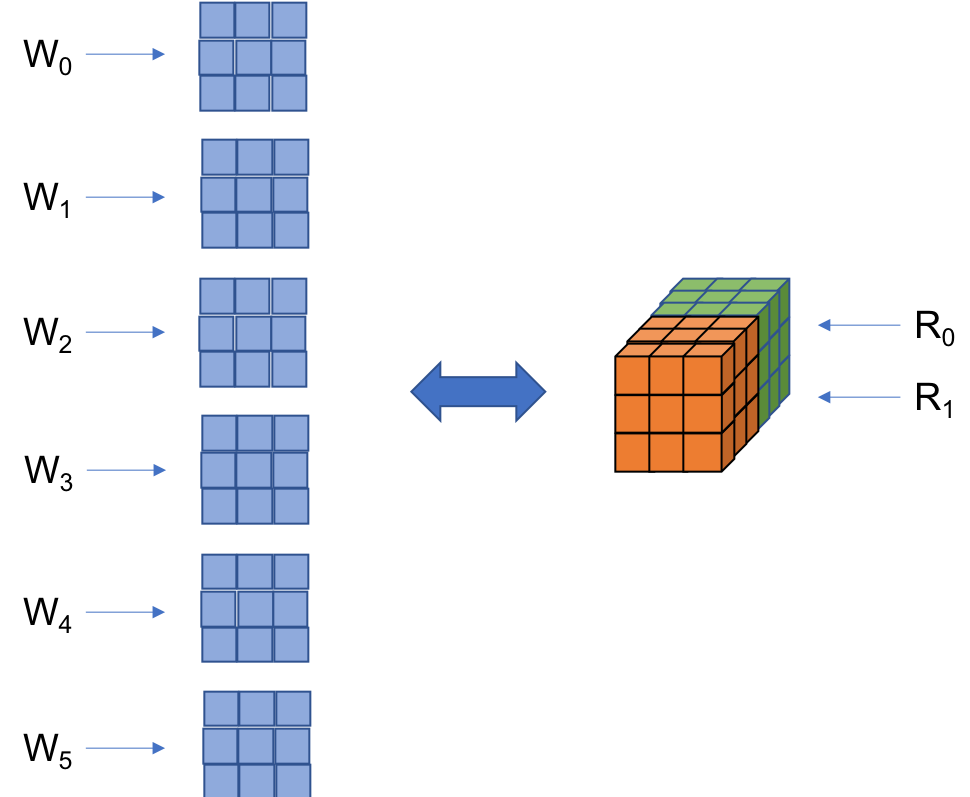
\includegraphics[bb= 0 0 600 400]{figs/write_read_locals.png}
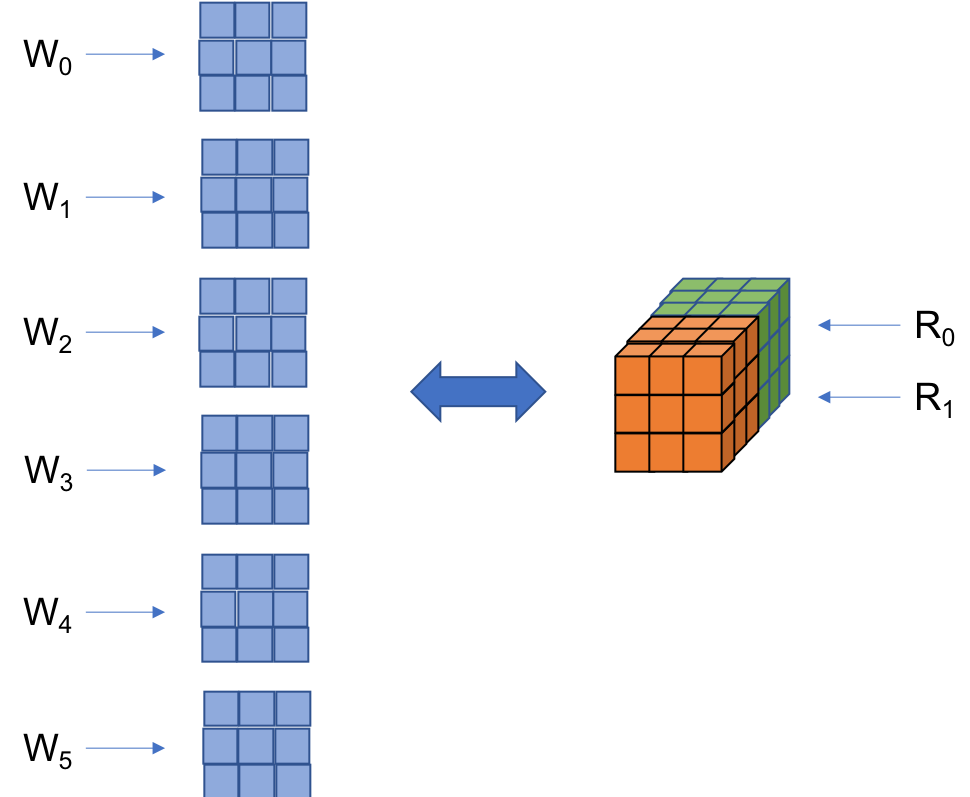
\includegraphics[width=3in]{figs/write_read_locals.png}
\caption{Local 2D arrays written by individual processes ($W_0-W_5$) appear to readers ($R_0-R_1$) as part of a 3D array where one array dimension represents writer id.}\label{fig:read-write-locals}
\end{wrapfigure}
The key to understanding this is the core ADIOS data model, which we describe as the Streaming Structure of Parallel Arrays (SSOPA).  The base query model that SSOPA offers is very limited -- one can identify a range of values that one wants from a global array, a range of values from a local array on a particular writing process, a global variable value, or a variable that had a different value on each writing process.  For each of these ``local'' values, ADIOS presents them as ``courtesy'' global arrays, where one dimension is simply the index of the writing process. 

This extension of the Structure of Arrays (SOA) approach to data, but using the distributed/parallel concept of arrays, is what gives us the key reading abstraction for scientific data.  The interface forces each write of data from an individual component to tag its patch with the offset and extent of the local patch within the global array, which allows us to offer a best-of-both-worlds view to the subscribers -- a Structure-of-Arrays model, where you can explicitly request a view on the arrays using simple offsets, and yet performance similar to array of structures, since each writer's block of data is maintained as an individual column store for efficient access.  Figure~\ref{fig:read-write-locals} is a schematic view of how the data looks to the publisher and the subscriber, each of which is individually a parallel code.



Concretely, this allows the interface to respect the fact that these extremely large data streams are composed of simultaneously delivered, distributed data shards. Naïvely, one could think of a large array of processes, each writing out a small patch of a large, distributed matrix. Performance in writing comes from the fact that we can make independent progress; the performance in reading the data leverages many of the same observations of performance of column stores vs row stores in database shards.  

The last key to the model is that the stream of parallel arrays has explicit synchronization windows, or ``steps'' in  ADIOS terminology. The sequence of these steps can be applied by a user in a number of ways -- as versioned partial updates to a table, as separators between distinct items like image data, or as the sequence of time step data from a simulation or experimental science campaign. The last of these is most common for our extreme-scale science community, but all of these engineering choices are supported through the abstraction. This explicit consistency marker by the publishers of the data give the runtime system flexibility for making performance decisions; different engines (as described in \S\ref{sec:coupling}) within ADIOS can implement lazy or imperative consistency as best fits their particular use case.

All together, the SSOPA model represents a base layer for the query model that has broad consensus among our user base.  On-going work explores extensions of the query model and the ADIOS API in a number of ways. Staying true to the requirement for adaptability in the ADIOS interface means that we must always be evaluating new ways to tune and extend the subscription interface. However, the logic of the base model and matching challenging user requirements always guides our development process. 
The modular execution approaches enabled by the SSOPA model help address the needs from across the developing exascale science frontier. 

% The value of the extended publish/subscribe model and the particulars of the SSOPA subscription interface are best understood in the context of the science cases that they enable. 



% \begin{figure}
% 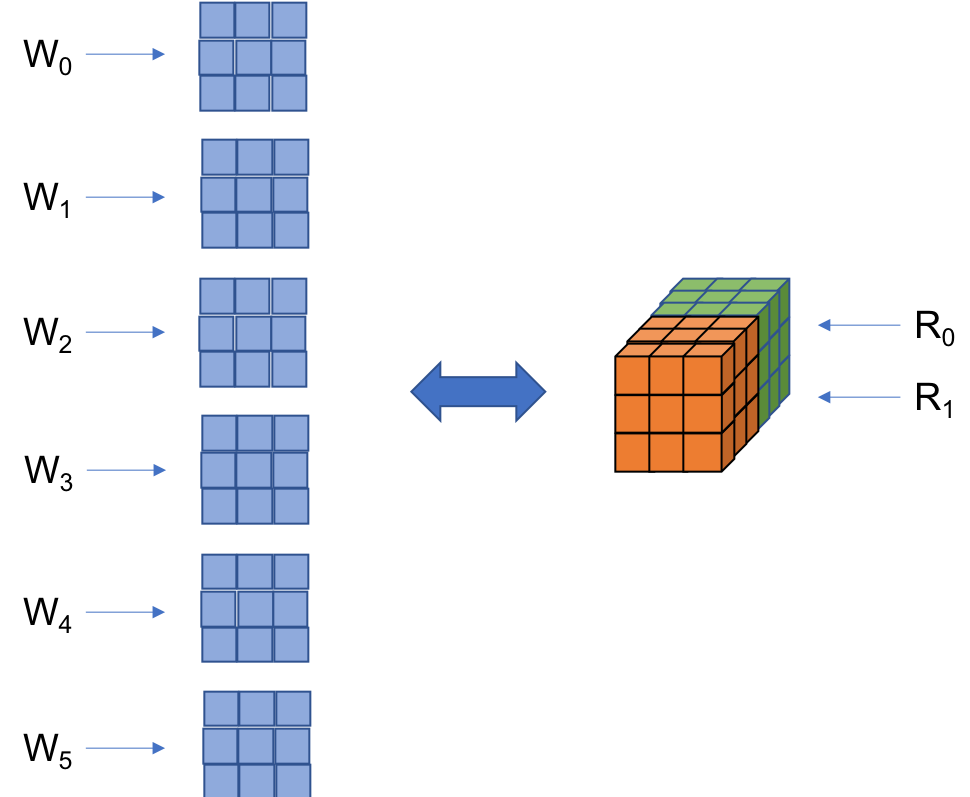
\includegraphics[bb= 0 0 144 81]{figs/write_read_locals.png}
% \caption{A simple figure.}
% \end{figure}




% Further, the range of data types that need to be correlated for an individual scientific campaign may range across a wide variety of sensor, simulation, analysis, and visualization data.  As we look to the arrival of the exascale platforms, we have had to make a number of changes to our data management platform, in order to extend it to address these incoming needs.

%\todo[inline]{End by making clear the connection to provenance, HOARDE, how that connects to relational databases, future directions, 5 V's, etc.}

%\todo[inline]{Need to fix missing references in this section}

\section{Near Exascale Science Use Cases }
\label{sec:usecases}
 Scientific computing has ridden along on the swell of interest in Big Data, and it is useful to use the lexicon of the 5 V's (Volume, Velocity, Variety, Veracity, and Value), as it helps to highlight where some of the key differences are that have caused divergence in the solutions that different communities use.  Although exascale computing does promise large volumes of data, that data is not like the data that drives internet-scale development.  Individual data elements are themselves extremely large (multiple TBs in size), and they arrive as part of tightly synchronized, high velocity bursts.  
 %The use cases we describe below (\S\ref{sec:usecases}) highlight that data management, and the software development process of the data managers, has been forced to step away from the monolithic designs for both code and data. 
 We have identified three examples of science teams that are preparing for the exascale era -- some in terms of exaflop computations, and others in terms of exabyte data -- that can help put the capabilities we discuss in \S\ref{sec:capabilities} into context, as well as further clarifying how ADIOS's data model addresses their core data management needs.


    
\subsection{Computational Fusion }


XGC is advanced fusion software designed to model plasma edge physics in magnetic confinement devices and one of the largest scientific simulations running at Department of Energy Leadership Computing Facilities (LCFs). 
XGC has demonstrated full-machine scalablity at the largest available sites, with jobs that result in multiple petabytes of data per hour over tens of hours durations. Such data generation already challenges the capacities of the file systems of current LCFs, and next generation machines will beckon even larger datasets. 
%Data types vary, including particles, five-dimensional distribution functions, and three dimensional fields on an unstructred mesh.
 At these scales, it is no longer feasible to store all relevant datasets and carry out post-simulation analysis only; the time to retrieve the quantity of data from disk/tape is too great. Output from an XGC simulation must be processed \textit{in situ} and in-transit through complex workflows for meaningful data reduction (before being written to storage) and for scientific data analysis and visualization.

Another I/O challenge facing fusion simulations is code coupling for Whole Device Modeling (WDM). By running multiple application codes concurrently, each focusing on a specific spatial region or physical phenomenon of the fusion device, researchers are building a holistic model to understand complex plasma reactions throughout the entire reactor. 
Execution of multiple fusion simulation codes with both tightly and loosely coupled data sharing during execution is needed. ADIOS provides performant data exchange methods to satisfy the various requirements.

Various I/O research leveraging ADIOS has been conducted to support data exchanges for loose and tight coupling scenarios, data reduction with strictly bounded physics properties, and efficient metadata management with high concurrency. Runtime performance research is necessary to insure that the coupled simulation is resilient to jitter caused by external network contention and unexpected system abnormality, and to provide online guidance through low-latency performance monitoring and prediction.

\subsection{Molecular Dynamics with LAMMPS  
%\textcolor{red}{- Lipeng/Matthew}
}


%\todo[inline]{Someone who knows molecular dynamics better than Eric should look over how I cleaned this up}

%The challenges in molecular dynamics and materials science modeling more generally are evolving. While simulations with millions, billions, and even trillions of atoms are now possible, often times this sort of scaling is no longer the primary impediment. 

Future molecular dynamics/materials science computing addresses
modeling on longer time scales; in particular, understanding
how we can design and manipulate materials so that their
long-term behavior meets our needs and requirements. 
Using the LAMMPS molecular dynamics code~\cite{LAMMPS},
researchers have begun studying problems such as the following:
What alloy mix is most likely to maintain integrity over two 
decades of radiation bombardment in a fusion reactor?
What mix of elements will best ensure that
radioactive elements are fully contained by a glass matrix 
protection from the outside world and the human population?

In general, improved flexibility, durability, and hardness 
over time are all achievable through better design and
manufacturing; however, traditionally the simulations do not
explore the breadth of possibility, focusing on a more limited 
range of the solution design space.
%The challenges in molecular dynamics and materials science modeling more generally are evolving. 
While simulations with millions, billions, and even trillions
of atoms are now possible, particle number scaling is
not the only difficulty --
%the simulations only progress based on what we ask them to study, rather than helping us to explore all of the opportunities that might exist.
long-time runs combine scalable performance with the management and control of concurrently-running ensembles of such runs. 
% The ensemble approach is required to
% to implement the time evolution of such classes of such materials.

%Working with the LAMMPS molecular dynamics code~\cite{LAMMPS}, researchers are studying phenomena that require not massive numbers of atoms, but instead require extremely long time scales -- if I want to design a material to line the inside of the ITER fusion reactor that will maintain integrity over two decades of radiation bombardment, what alloy mix is most likely to last that long?  If I want to trap nuclear waste in a glass prison to protect people for thousands of years, what mix of elements will make sure the radioactive elements can't escape the matrix?  These sorts of questions require techniques that combine scalable performance of the molecular dynamics control as well as regular exchange and management of collections of ensembles of such runs.  Only through using the ensemble approach can we try to see the time evolution of such classes of such materials.

The I/O challenge for such scenarios is multi-faceted.  At a base layer, one needs to accelerate the performance of each individual parallel run as much as possible.  On another level, one must collect, calibrate, and make decisions upon the sets of such time-stamped data in order to direct exploration of the evolution of the system.  For that to be efficient, in-memory streaming of data is needed for runtime coupling, even if the development, testing, and validation needs those same interfaces to work through file I/O.  Finally, with the extent of the number of ensemble members, it is critical to manage the metadata representations so that one can not only query based on computational provenance (i.e. Run \#23478) but also on location (i.e. on the burst buffer) and on relevant features (i.e. after the crystal cracked).  


% \subsection{Particle Accelerators \textcolor{red}{- Norbert  }
% }
% PIConGPU, openPMD and moving to AMR.




\subsection{Radio Astronomy with The Square Kilometre Array
%(Federated Science, Performance) %\textcolor{red}{- Jason }
}

Radio astronomy data is another major use case of our I/O abstraction model. In particular, we have been focusing on data I/O challenges of the future world's largest radio telescope, the Square Kilometre Array (SKA).  SKA is an international project that will offer unprecedented views to the astronomy community.  From a data perspective, it is an intimidating challenge -- in the initial phase, the output from more than 130,000 antennas located in Western Australia will be streamed, condensed, analyzed, and then fed into an open science repository.  In the initial phase, this will be at 10 Tbps, with over an order of magnitude increase in bandwidth requirement expected as the SKA platform fully comes on line~\cite{WANG2019}.
%\todo[inline]{explain what this is from the exascale data management perspective -- observational, high velocity, global community data}

One of the most difficult I/O challenges for the radio astronomy community is storing visibility data. It is generated at an early stage in the typical data reduction pipeline, and it is usually the largest data product across the entire workflow. For the past two decades, most such data has been stored in the MeasurementSet format through the Casacore Table Data System (CTDS) \cite{DIEPEN2015}. CTDS was designed under the assumption that most radio astronomy data processing algorithms can be embarrassingly parallelized, and it does not use parallel I/O. 
%This had been working properly with most of the radio telescopes until SKA came into view. 


CTDS has been sufficient for most radio telescopes prior to 
SKA. However, SKA will have orders of magnitude more antennas than previous radio telescopes, and the volume of visibility data scales quadratically with the number of antennas. 
%This data volume may not lend itself well to a serial I/O system and the embarrassingly parallel paradigm. 
In order to better understand the potential bottlenecks, we have simulated the full scale SKA Phase 1 Low data using most compute nodes of the world's fastest supercomputer, Summit~\cite{WANG2019}. The results showed that the embarrassing parallel model is no longer optimal when scaling up to the full-scale SKA level,
possibly explainable by producing too many small table files,
which bottleneck the parallel filesystem.

%Part of the reason, which we are still investigating, may be because that it produced too many small table files, which hit the bottleneck of the parallel filesystem.

We have developed an ADIOS storage manager for CTDS, which
enables parallel I/O for CTDS at the column
layer, and repeated the SKA workflow using it \cite{WANG2016}.
%We have also tried running the workflow using the ADIOS storage manager \cite{WANG2016} that we have developed for CTDS, which enables parallel I/O for CTDS at the column layer. 
The performance is at least one order of magnitude better than the embarrassingly parallel model even at the partial SKA Phase 1 scale. However, due to limitations of the CTDS architecture, we have yet to enable parallel I/O at the table layer, which would likely improve performance even further. Doing so will also require optimizations at the metadata management layer that we will discuss in \S\ref{sec:capabilities}, in order to handle table-based data more efficiently.

\subsection{Lessons Learned}

The science use cases described above highlight several important challenges for exascale computing. 
The extreme data sizes being handled by the Computational Fusion and the Radio Astronomy examples will require new reduction and compression capabilities, which we discuss in~\S\ref{sec:reduction}.
Both the Fusion and Molecular Dynamics cases call for robust coupling mechanisms for a variety of coupling situations, as we describe in~\S\ref{sec:coupling}. All three science examples point to the need for integrated tools for runtime performance understanding, a capability that we examine in~\S\ref{sec:performance}. Finally, the complexity of data in the Molecular Dynamics case and the Radio Astronomy case both point to the need for specific metadata management capabilities, which we detail in~\S\ref{sec:metadata}.


\section{Capabilities for Exascale 
%- 1 pg. each
}
\label{sec:capabilities}

There are many specific technical approaches and results that have been developed in response to these science needs.  What we summarize here are the broader core capabilities that we have identified as being required to address the needs of these science applications in the exascale era.  For each of these capabilities, we have tried to highlight specific papers and projects that one can explore for greater technical detail.
%Each of them in turn addresses key components of the extended publish/subscribe semantics as you address the scientific data management needs.

%\todo[inline]{Here we explore various capabilities that will be required for extreme scale computing, and discuss how we are providing these capabilities in ADIOS.  Be sure to focus on the capability first and why it's useful for addressing exascale problems/technologies, and then the particular tools/demonstrations just showcase how we're trying to fulfill those capability requirements.}
%\todo[inline]{Need intro to describe the connection between lessons learned and the capabilities below.}

\vspace{10px}
% \todo[inline]{
% Guide for each section:

% \begin{enumerate}
%   \item Select feature of science case(s)
%   \item Exascale gap/new requirement for capability
%   \item Comparison to state of art
%   \item Design and partial results of addressing it in ADIOS
% \end{enumerate}

% These aren't necessarily subsections, but try to be sure that you clearly hit each of those beats.  Probably a paragraph apiece for the first three, and then 2-3 paragraphs and a figure for the final part.




\subsection{Reduction and Compression Capabilities %\textcolor{red}{- Scott,  (Kshitij, Jieyang, Gary, Nick, Mark A., Ben)}
}
\label{sec:reduction}

%The Sirius story~\cite{klasky2016exascale}

%\begin{center}
% \begin{wrapfigure}[5]{L}[0pt]{1.75in}
% \vspace{-15pt}
% \begin{tcolorbox}[width=1.7in,
%                   %%enhanced,
%                   boxsep=1pt,
%                   left=0pt,
%                   right=0pt,
%                   top=2pt,
%                   ]%%
%  \begin{center}
%  \begin{quote}
%     {\em The purpose of computing is insight, not numbers. } \\ --Richard Hamming
%  \end{quote}
%  \end{center}
% \end{tcolorbox}
% \end{wrapfigure}
% % \end{center}

\begin{wrapfigure}[5]{L}[0pt]{2.9in}
\vspace{-15pt}
\begin{tcolorbox}[width=2.85in]
 \begin{center}
 %\begin{quote}
    {\em The purpose of computing is insight, not numbers.} \\ --Richard Hamming
 %\end{quote}
 \end{center}
\end{tcolorbox}
\end{wrapfigure}
% \end{center}
 
 Richard Hamming's remark~\cite{Hamming:book}, made over 50 years ago at the dawning of the age of large scale scientific computation, is even more relevant today as we prepare for scientific simulation at exascale. Avoiding bottlenecks in exascale scientific discovery requires
research into managing, storing, and retrieving the large volumes of data that are
produced by simulations and analyzed for months afterwards. Our main objective is to accelerate knowledge discovery, and as data sizes grow from 
simulations and experiments, it is imperative that we prioritize information over
data.  

Some of the fundamental research we have done aims to manage the overall data life cycle, including data generation (e.g., from a simulation) or acquisition (e.g., in the case of experimental and observational data), optimized data placement, runtime data management including migration, reorganization and reduction, data consumption for knowledge discovery, and purging data from the system to optimize system operation. 


The classical workflow where the entire dataset is written to storage for later analysis will no longer be viable at exascale, simply because the amount of generated data will be too large due to capacity and performance limitations. 
In the future, it will be vital to take advantage of \textit{a priori} user information (1) to gain higher performance and predictability of I/O, (2) to prioritize the most useful data for end users so that I/O can be finished under time constraints, and (3) to perform \textit{in situ} operations and analysis before storing the information.
A result of these requirements is a need for a set of techniques to reduce and restructure data, here referred to as Data Refactoring. In recent years, libraries such as SZ\cite{sz2}, ZFP\cite{zfp2}, MGARD\cite{ainsworth2018multilevel} have emerged as leading techniques for compressing and reducing large, voluminous data at extreme scales.
The research using MGARD is an important part of the response to this need for data refactoring.  It is a progressive compression technique, based on the theory of multigrids, that allows one to segment data into components that can be individually managed and yet also can bound the error and timeliness of your read request by only pulling the number of components from the multigrid layers that are needed for the accuracy at hand.



The challenge when applying refactoring techniques, particularly application-aware techniques, is how to incorporate sufficient knowledge in the storage system such that an arbitrary future client has sufficient information to recreate the desired information. Additionally, by spreading data across multiple different kinds of storage media that typically have independent namespaces, locating any particular data will be challenging.


\begin{wrapfigure}[14]{R}[0pt]{3.5in}
\begin{tcolorbox}[title={Key research questions addressed by ADIOS with MGARD}]
\begin{enumerate}
    \small
    \itemsep-0.4em
    \item How can we initially place data so that it can be discovered and consumed efficiently?
    \item How can the placement and migration of data across a multi-tiered storage hierarchy be optimized at runtime, both from the application and system perspective?
    \item How can knowledge about the application used to better prepare the data for consumption?
    \item When and how do we make the decision to purge data?
\end{enumerate}
\end{tcolorbox}
\end{wrapfigure}

\textit{A priori} information can be provided by application scientists regarding which data should be sent where in the storage system (so that minimally, the most science-relevant data can be available for subsequent analysis. This can allow science goals to be accomplished even when the storage is busy servicing other users. 

For our approach, data refactoring generates the needed prioritization classes. There are many data refactoring techniques, including re-organization and reductions, and the best choice will generally be application- and user-dependent. However, our observation is that, once the choice is settled, it will not typically change from run to run within an extended campaign.
One research challenge in effectively and efficiently refactoring data is understanding when the time and resources required to identify and execute the “best methods” exceeds the gains achieved. Another critical question concerns quantifying and controlling information loss due to refactoring the data and using a reduced dataset. Broadly speaking, the path from data to knowledge consists of extracting underlying models or patterns from the datasets and interpreting the resulting models. Although scientific data generally contains random components due to finite precision and measurement and calibration effects, useful scientific data is never purely random. As such, a core concern in refactoring is understanding how much information is present in a data set and therefore which type(s) of refactoring will be most effective. 

Ideally, scientists would like to perform the entire analysis \textit{in situ}, thus avoiding intermediate data sets and effectively circumventing the large data issue completely. The catch, of course, is that this is unlikely to achieve the best science results since, by their nature, large-scale simulations aim to discover new and emergent behavior often hidden in the form of higher order effects within the data deluge. In particular, this means if data thinning or truncation is applied haphazardly, the higher order information sources may be eliminated. 
Typically, entire data sets cannot be stored in easily accessible storage due to its sheer size. However, the data cannot be reduced prior to archiving without risking losing information. Viewed in this way, the problem would appear intractable. As noted above, though, this is not a true impediment as long as we can incorporate a user’s \textit{a priori} knowledge of models and effective refactoring techniques.  The information needed to answer the scientist’s particular science goals is frequently significantly smaller, and using careful information-theoretic and application-given techniques the Storage System and I/O layer can exploit this. In situ data management and reduction pipelines comprise of multiple steps: applying reduction techniques, assessing the quality of reduction, analyzing data to ensure preservation of essential features, and assessing the overall performance of the full pipeline.

Deep application knowledge means one can sometimes achieve dramatically superior data reduction compared with what one might achieve otherwise. However, even in the absence of such high level knowledge, an I/O system must offer generic data reduction and re-organization techniques. For instance, certain basic data semantics information is needed and must be supported by the overall infrastructure. Effective \textit{in situ} data management is a vital component of overall large data management at the exascale.


\subsection{Coupling Capabilities %\textcolor{red}{- Greg (Norbert, Jason, Matthew)}
}
\label{sec:coupling}

Another way to understand ADIOS's publish/subscribe view\cite{Flexpath,choi2018} is to recognize that from the perspective of data producers and consumers, everything is coupled via these publish/subscribe channels. It is the user's choice at runtime to choose a service provider, ``engine'', that dictates whether this coupling happens asynchronously through files, synchronously through memory, or in a more complicated pattern. Table~\ref{tab:engines} showcases some of the available engines as of ADIOS 2.5.
% In ADIOS, inter-application communication is accomplished using
% the same basic API that is used for reading and writing to files.
% However in the case of coupled components, ADIOS data written in one component
% is instead made available as an item to be read in another component.
Though this simple description of functionality belies a host of complexity,
%in the ADIOS ``Staging Engines'', the subset of engines that focus on concurrently-executing components. 
the basic functionality of managing the data exchange defined by the SSOPA model is shared by all engines.
%but beyond that, the staging engines vary in functionality and focus.


\begin{table}
\begin{center}
\footnotesize 
\rowcolors{2}{gray!25}{white}
\begin{tabular}{ | m{7em} || m{15em}| m{15em} | } 
\hline
\rowcolor{gray!55}
Staging Engine & Characteristics & Application Domain \\ 
\hline \hline
SST & Configurable queueing, dynamic connections, multiple readers, WAN and RDMA &  General use\\ 
\hline
SSC & MPI-based coupling & Optimized for tightly coupled simulation codes utlizing MPI. \\ 
\hline
BP4 & File-based coupling, readers update as file is written  & Useful for development and temporal analysis\\ 
\hline
Inline & In-process coupling, zero copy data delivery & Requires specially written applications, only $N\rightarrow N$ coupling\\
\hline
\end{tabular}
\caption{ADIOS2 Staging Engines} \label{tab:engines}
\vspace{-25pt}
\end{center}
\end{table}


While all of the science cases above share a need for direct communication between
running HPC programs, they do differ in the details of their needs and the nature 
of the data exchange required.  For example Whole Device Modeling requires bi-directional coupling between components and the 
simulation for timestep $N+1$ in any component application cannot proceed without 
the data produced by timestep $N$ in other coupled applications.  We refer to this
level of interdependency as ``strong coupling'' and in this case the staging system
often has very little flexibility in meeting the application communication needs, 
as any latency or bandwidth limitations have a direct impact on the performance 
of the composite application.  In contrast, other coupling situations are ``weak''
and allow the communication system more flexibility.  In LAMMPS for example, 
the simulation and the analytics form a simple pipeline, and while the performance 
of that pipeline is important, there are also opportunities for techniques such 
as queueing and latency hiding that can enhance the overall performance of the
system.

To support the strongest coupling cases, where all participating components can 
share a global MPI communicator via MPI's MPMD launch mode and the application
communication pattern is fixed, ADIOS features the Strong Staging Coupler (SSC)
engine. In the first timestep, SSC records the geometry of the SSOPA exchange between the coupled components (what array elements are written and read where), and on
subsequent timesteps that data exchange is re-enacted using one-sided MPI put 
and get calls.  This fixed pattern of data exchange is not a universal feature 
of HPC applications, but it does appear in important subsets, such as XGC, and
relying upon it allows SSC to exploit highly-optimized MPI implementations on 
emerging exascale computing platforms.

In situations where the coupled components cannot meet the criteria necessary to use SSC, ADIOS users can fall back to another staging engine, the Sustainable Staging Transport (SST).  Unlike SSC, SST uses MPI only within each application, so it doesn't require all components to be launched simultaneously with MPMD mode and uses one of several non-MPI transports to move data between applications.  Currently those transports include a LibFabric-based RDMA transport for intra-cluster use, TCP- or UDP-based transports for inter-cluster or WAN communication and an experimental shared-memory transport.  In support of the pub/sub model described in this paper, SST supports dynamic connection and disconnection of Reader clients, including multiple simultaneous readers.  This is an important feature for visualization clients that may wish to connect and disconnect from a running analysis application, but it also has a variety of other uses, including making sure that something like the failure of a connected analysis application doesn't interfere with an ongoing simulation.  Also unlike SSC, SST doesn't assume lockstep synchronization between readers and writers, instead it buffers timestep data until it is required, transmits the data to readers when requested, and manages the release of buffered data after it is consumed.  Because unbridled queuing can lead to memory exhaustion and some applications have little memory to spare for staging, SST also has mechanisms for limiting queue sizes and allows applications to either block or discard data on queue full conditions.  Like SSC, SST can also take advantage of fixed communication patterns for the purpose of pre-loading data to the readers where it will be consumed.  

While the basic design of ADIOS coupling has been flexible enough to support high performance publish/subscribe operation in today's critical applications, we anticipate changes to support the needs of emerging applications and systems.  Some of these changes, like managing performance and placement as data moves through more complex storage hierarchies, likely fit within current ADIOS APIs and semantics.  However, additional techniques borrowed from pub/sub systems, such as the writer-side filtering and data reduction offered by derived events\cite{Eisenhauer2006}, may require reimagining the nature of ADIOS read semantics.


\subsection{Performance Understanding 
%\textcolor{red}{- Jeremy (Jong, Matthew, Kshitij)}
}
\label{sec:performance}

%\textbf{Select feature of science case(s): }
Exascale computing will bring us unprecedented computing performance through massive new machines involving both a vast collection of CPU cores as well as cutting edge GPUs, all connected through extremely fast and flexible networks and leveraging a range of new memory and storage technologies. With well tuned codes, these machines will be capable of exascale performance, but balancing the CPU / GPU mix, and avoiding network misuse and storage bottlenecks will be more important than ever. In addition to the raw scale of the machinery, the science cases described in \S\ref{sec:usecases} demonstrate a range of behaviors that drive new performance needs which are difficult to meet with conventional software technologies. In particular, we have seen a change from the construction of single, monolithic codes to computational experiments composed of multiple executables, run as ensembles, coupled codes, or as pipelines of \textit{in situ} computations. We also observe increasing need for federated computing where, for instance, large data sources such as accelerators and radiotelescopes are used to feed extreme scale computing resources that are geographically separated from the data sources. This will require that these application be tuned not just within a single supercomputer, but with tuning strategies that span multiple sites and platforms.

The tools that have been built up over the last decades for performance understanding and management of large MPI-based codes are capable primarily of static, post hoc analysis of application performance. But this style of analysis will not be sufficient for application workflows with many moving parts and requiring careful orchestration of those parts to achieve adequate performance on complex hardware platforms. Runtime availability, aggregation, and analysis of performance information will be critical for such orchestration, as will the ability to accurately model~\cite{wanhpcc2017} and predict the performance of application components, and place processes appropriately~\cite{choicluster2017}.
Systems will need to address many additional constraints and concerns as a result of dealing with the measurement of collections of distinct runtimes and distinct applications, and it becomes more than what a simple patchwork of fixes can address.


%\textbf{Comparison to state of art: }
Existing tracing and profiling tools and frameworks such as Scalasca~\cite{geimer2010scalasca}, ScoreP~\cite{scorep} and Tau~\cite{Shende2006tau} tend to be batch oriented, with a focus on post-mortem analysis, and typically operate on a single process or MPI application. Existing runtime techniques do not offer detailed aggregate views of the performance of a suite of concurrent applications. As a result, it is difficult to get the holistic view needed at runtime for coupled codes or ensemble suites using these types of tools.

%\textbf{Design and partial results of addressing it in ADIOS}
As we examine the needs of exascale performance understanding, it is clear that a variety of performance metadata from tracing and profiling must be made available at runtime. As some of these measurements can be expensive, we must have the ability to turn individual measurements on and off as needed, and to adjust frequency of measurements, and delivery criteria. At first glance, it would appear that the pub/sub tools might directly support the additional performance metadata through the same mechanisms that handle application data, however the delivery requirements of performance metadata may be quite different from those of application data, not only in terms of destination, but also delivery frequency and latency. So care must be taken not to carelessly mix data and performance metadata, but rather to allow out-of-band approaches for expediting performance metadata when necessary. Such tools must provide appropriate flexibility while remaining user friendly and avoiding the introduction of network bottlenecks.

In~\cite{mona2019}, we presented a prototype system for collecting and aggregating performance data. The system leveraged the Tau software for tracing and profiling, and introduced an aggregation layer capable of merging this performance metadata collected across a large number of nodes into a single global view that could be queried by performance analysis components at runtime. 
This work demonstrated several examples of leveraging runtime performance information, including runtime application monitoring, I/O model extraction, understanding I/O variability, and dynamic process placement.
As an example of the use of this sort of monitoring infrastructure, Figure~\ref{fig:variability} illustrates the variability inherent across and within runs of XGC-1 on both Titan and Theta. 



\begin{figure}[tbh]
\vspace{-10pt}
\center
\subfloat[][Titan]{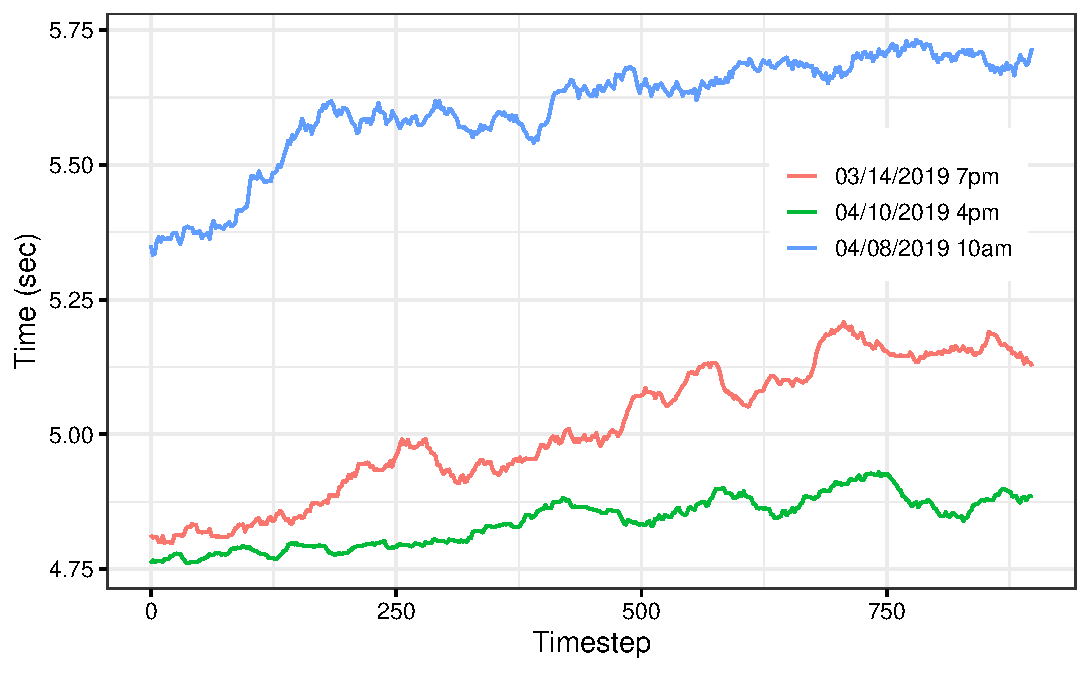
\includegraphics[width=0.45\textwidth]{figs/var-titan.pdf}}
\subfloat[][Theta]{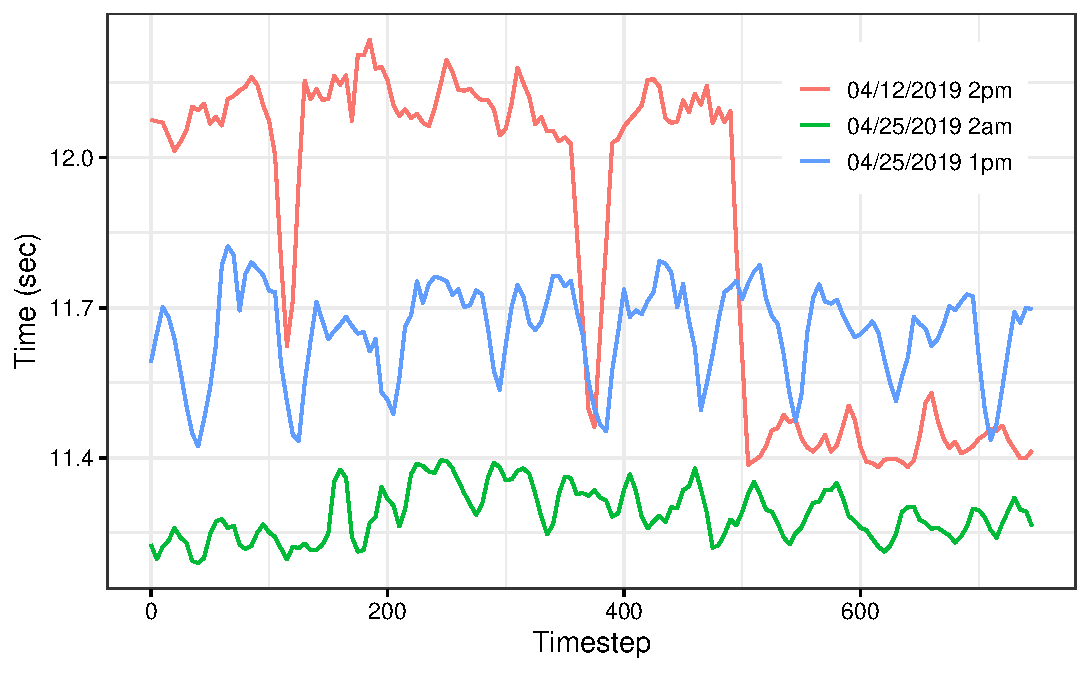
\includegraphics[width=0.45\textwidth]{figs/var-theta.pdf}}
\caption{Performance variability of XGC-1.  The results presented here for Titan (a) and Theta (b) show the degree of variability in performance both within a timestep and across separate runs.}
\label{fig:variability}
\end{figure}





%Leverage publish/subscribe to allow components to subscribe to performance data as needed. Allows monitoring system to offer a wide range of detailed measurements, but perform only the measurements that are requested by subscribers.
%Challenging because performance data will require different handling than application data. lightweight, out of band...


\subsection{Metadata Management Capabilities 
%- \textcolor{red}{Lipeng (Norbert, William)}
}
\label{sec:metadata}

In order to make scientific data
%the data produced by scientific applications 
easy to retrieve, reuse and re-evaluate over its lifetime, plenty  of  metadata  
%associated  with  the  raw  values are 
is also generated. For example, a simulation 
%running 
with thousands of MPI processes for millions of steps needs to output data every 100 or 1,000 steps. The output data contains variables that are global arrays and each MPI process is a writer which outputs a specific block of each global array. In this case, we need metadata for each block to track which process generates it and at which simulation step, which variable it belongs to, where it is located in the global array, where to find it in actual file, etc.  As we can see, even for writing out a single variable, the amount of metadata needed can be huge. If a simulation outputs hundreds of variables, the  number of metadata items will further increase, which not only leads to extra I/O and storage overhead, but also exacerbates the computation and communication overhead since the metadata needs to be gathered and reorganized into certain format. In this subsection, we are going to discuss several specific metadata challenges we face when we design ADIOS. Some of these challenges have been well addressed which results in some unique capabilities enabled by current ADIOS implementation, while the others are planned to be addressed by future work.

First of all, in order to achieve better I/O performance on parallel file systems, scientists often let each MPI process of their simulation output its own data, which is usually a specific data block that is part of a much larger global variable. If the simulation data is generated in this way, it requires I/O libraries such as ADIOS to be able to efficiently manage the metadata for each data block. In ADIOS, this challenge is addressed by leveraging a log-structured file format called BP, which is the ADIOS native binary file format. In BP format, the data generated by each writer are organized and stored in a block by block manner. Specifically, each writer directly writes its own data blocks to the file system, while in the meantime it maintains each data block's metadata, which will be later gathered by a specific MPI process.
%(rank 0 in \texttt{MPI\_COMM\_WORLD})
 
This process organizes the metadata items collected from all writers into certain order and then writes them into the metadata file. Moreover, the metadata contains not only the information for locating each data block, but also some characteristics, such as minimum and maximum value,  of each data block, which enables the capability of building a fast query interface. Or in other words, users can query the characteristics of each data block without touching the actual data as those characteristics have been included in the metadata.

Second, there are different ways to organize metadata items collected from all writers, the challenge is to not only reduce the communication and computation overhead of gathering and organizing the metadata items, but also provide users some flexibility so that different data access patterns can be supported. In order to reduce the overhead of constructing global metadata, 
%when we design BP format, 
we separate the metadata items of each simulation step from each other and build an extra index table to locate them in a step-by-step manner \cite{Wan:2019}. This also allows users to access data generated at any simulation step without parsing the metadata of all previous steps, which is especially useful for data streaming use cases, such as online analysis and code coupling. Moreover, since the index table is small and can be easily loaded into memory of each reader, querying metadata of each simulation step is an atomic transaction which enables lock-free data access for asynchronous readers. 

As future work, we need to address two critical challenges in metadata management for scientific applications. One is to further reduce overhead of constructing metadata when simulation outputs a plethora of variables with complex attributes. The other one is to support data query across multiple storage tiers. With the development of data storage technology, HPC systems are equipped with complex I/O subsystems that usually consists of multiple storage tiers. For instance, besides center-wide parallel file systems and tape storage systems, all DoE's leadership supercomputers have an intermediate storage tier called burst buffer.
%, which are either dedicated I/O nodes equipped with SSDs or non-volatile memory devices attached to each compute node
Scientific applications might write data to all these storage tiers based on their needs. Therefore, it is critical to design an efficient metadata mechanism that can track data objects and accelerate data movement across all storage tiers.


\section{Conclusion}

Exascale computing is bringing new usage patterns that will open up new areas of scientific discovery. The traditional monolithic simulation code is being replaced with coupled codes, \textit{in situ} workflows, and large ensembles of independent tasks. In the face of these new usage patterns, bespoke custom workflows are becoming increasingly unwieldy. Monolithic solutions are unlikely to be suitable, as portions of workflows will need to be performed across different resource scales. Systems that provide efficient and reusable support for the new usage patterns are needed.

The publish/subscribe metaphor provides a good starting point for designing such systems to accommodate the I/O and data management needs of the exascale era. ADIOS as an Adaptable I/O System based on the publish/subscribe paradigm has been used to support some of these emerging data needs.  New usage patterns will require that new capabilities be added to existing pub/sub mechanisms. Compression and reduction capabilities, like MGARD, will be required to deal with data volumes that continue to outpace memory and storage capacity of new systems. Efficient coupling capabilities are needed to support new paradigms of application coupling and \textit{in situ} composition. Extensions to performance monitoring capabilities will enable the advanced monitoring and tuning that will be needed to keep exascale machines fully utilized, and careful adjustments to metadata management systems are needed to insure that application access patterns can be supported efficiently. As new exascale systems come online, ADIOS will continue to adapt to the changing landscape of high performance computing in order to meet new application needs.
%\todo[inline]{Bring it home, Greg! ... as Baby Yoda once said...}

% New technologies inspire changes in the way applications are structured which in turn inspires more changes in technology.  
%\begin{center}\begin{tcolorbox}[width=4in, hidden,interior hidden,boxsep=0pt,left=0pt,right=0pt,top=2pt,]\begin{quote}\begin{center}{\em “So long, and thanks for all the fish.”\\― Douglas Adams}\end{center}\end{quote}\end{tcolorbox}\end{center}


\paragraph*{Acknowledgment}
Without the continued support from the Department of Energy's Office of Advanced Scientific Computing Research, the projects upon which this future vision rests would not be possible. This research used resources of the Oak Ridge Leadership Computing Facility, which is a DOE Office of Science User Facility supported under Contract DE-AC05-00OR22725, as well as resources of the National Energy Research Scientific Computing Center (NERSC), a U.S. Department of Energy Office of Science User Facility operated under Contract No. DE-AC02-05CH11231.


%TODO: Move from bibtex to the following:
\begin{thebibliography}{10}
\setlength{\itemsep}{0pt plus 0.2ex}
\footnotesize

\bibitem{ainsworth2018multilevel} M. Ainsworth, O. Tugluk, B. Whitney, and S. Klasky.  \newblock Multilevel techniques for compression and reduction of scientific data---the univariate case. \newblock {\em Computing and Visualization in Science}, 19(5-6):65–76, 2018.

\bibitem{choi2018} J. Y. Choi, C. Chang, J. Dominski, S. Klasky, et al. 
%G. Merlo, E. Suchyta, M. Ainsworth, B. Allen, F. Cappello, M. Churchill, P. E. Davis, S. Di, G. Eisenhauer, S. Ethier, I. T. Foster, B. Geveci, H. Guo, K. A. Huck, F. Jenko, M. Kim, J. Kress, S. Ku, Q. Liu, J. Logan, A. D. Malony, K. Mehta, K. Moreland, T. Munson, M. Parashar, T. Peterka, N. Podhorszki, D. Pugmire, O. Tugluk, R. Wang, B. Whitney, M. Wolf, and C. Wood. 
\newblock Coupling exascale multiphysics applications:  Methods and lessons learned. \newblock In {\em 14th IEEE International Conference on e-Science, e-Science 2018, Amsterdam, The Netherlands}, pages 442–452. IEEE Computer Society, 2018.

\bibitem{choicluster2017} J. Y. Choi, J. Logan, M. Wolf, G. Ostrouchov, T. Kurc, Q. Liu, N. Podhorszki, S. Klasky, M. Romanus, Q. Sun, M. Parashar, R. M. Churchill, and C. S. Chang.  \newblock TGE: Machine learning based task graph embedding for large-scale topology mapping. \newblock In {\em 2017 IEEE
International Conference on Cluster Computing (CLUSTER)}, pages 587–591, Sep. 2017.

\bibitem{Flexpath} J. Dayal, D. Bratcher, G. Eisenhauer, K. Schwan, M. Wolf, X. Zhang, H. Abbasi, S. Klasky, and N. Podhorszki. \newblock Flexpath: Type-based publish/subscribe system for large-scale science analytics. \newblock In {\em 2014 14th IEEE/ACM International Symposium on Cluster,
Cloud and Grid Computing}, pages 246–255, May 2014.

\bibitem{sz2}  S. Di  and  F.  Cappello. \newblock  Fast  error-bounded  lossy  HPC  data  compression  with  SZ.   \newblock In
{\em 2016  IEEE  International  Parallel  and
Distributed Processing Symposium (IPDPS)}
, pages 730–739, May 2016.

\bibitem{Eisenhauer2006} G. Eisenhauer, K. Schwan, and F. E. Bustamante. \newblock Publish-subscribe for high-performance computing. \newblock {\em IEEE Internet Computing}, 10:40---47, 2006.

\bibitem{geimer2010scalasca} M. Geimer, F. Wolf, B. J. Wylie, E.
{\'A}brah{\'a}m, D. Becker, and B. Mohr.  \newblock The Scalasca performance toolset architecture. \newblock {\em Concurrency
and Computation: Practice and Experience}, 22(6):702–719, 2010.

\bibitem{Hamming:book} R. W. Hamming. \newblock  {\em Numerical Methods for Scientists and Engineers.}, McGraw-Hill, Inc., USA, 1973.

\bibitem{ViewfromORNL} S. Klasky, M. Wolf, M. Ainsworth, et al.
%C. Atkins, J. Choi, G. Eisenhauer, B. Geveci, W. Godoy, M. Kim, J. Kress, T. M. Kurc, Q. Liu, J. Logan, A. B. Maccabe, K. Mehta, G. Ostrouchov, M. Parashar, N. Podhorszki, D. Pugmire, E. Suchyta, L. Wan, and R. Wang. 
\newblock A view from ORNL: scientific data research opportunities in the big data age. \newblock In {\em 38th IEEE International Conference on Distributed
Computing Systems, ICDCS 2018, Vienna, Austria}, pages 1357–1368, 2018.

\bibitem{scorep} A. Kn{\"u}pfer, C. R{\"o}ssel, D. a. Mey, et al.
%S. Biersdorff, K. Diethelm, D. Eschweiler, M. Geimer, M. Gerndt, D. Lorenz, A. Malony, W. E. Nagel, Y. Oleynik, P. Philippen, P. Saviankou, D. Schmidl, S. Shende, R. Tsch{\"u}ter, M. Wagner, B. Wesarg, and F. Wolf.
\newblock Score-P: A
joint performance measurement run-time infrastructure for Periscope,Scalasca, Tau, and Vampir \newblock In {\em Tools for High Performance Computing 2011}, pages 79---91, Berlin, Heidelberg, 2012. Springer
Berlin Heidelberg.

\bibitem{zfp2} P. Lindstrom. \newblock Fixed-rate compressed floating-point arrays. Computer software. {\em https://www.osti.gov//servlets/purl/1231942}. Vers. 00. USDOE. 30 Mar. 2014. Web.

\bibitem{HelloAdios} Q. Liu,  J. Logan,  Y. Tian,  et al.
%H. Abbasi,  N. Podhorszki, J. Y. Choi,  S. Klasky,  R. Tchoua,  J. Lofstead,  R. Oldfield,  M. Parashar, N. Samatova, K. Schwan, A. Shoshani, M. Wolf, K. Wu, and W. Yu. 
\newblock Hello ADIOS: the challenges and lessons of developing
leadership class I/O frameworks. \newblock {\em Concurrency and Computation: Practice and Experience
}, 26(7):1453---1473, May 2014.

\bibitem{LAMMPS} S. Plimpton.  \newblock Fast parallel algorithms for short-range molecular dynamics. \newblock {\em Jrnl of Computational Physics
}, 117(1):1---19, 1995.

\bibitem{Shende2006tau} S. S. Shende and A. D. Malony. \newblock The TAU parallel performance system. \newblock {\em The International Journal of High Performance Computing
Applications}, 20(2):287---311, 2006.

\bibitem{DIEPEN2015} G. van Diepen.  \newblock Casacore Table Data System and its use in the MeasurementSet. \newblock {\em Astronomy and Computing}, 12:174---180, 2015.

\bibitem{Wan:2019} L. Wan, K. V. Mehta, S. A. Klasky, M. Wolf, H. Y. Wang, W. H. Wang, J. C. Li, and Z. Lin. \newblock Data management challenges of exascale
scientific simulations:  A case study with the Gyrokinetic Toroidal Code and ADIOS. \newblock In {\em The 10th International Conference on Computational Methods},  ICCM’19, 2019.

\bibitem{wanhpcc2017} L. Wan, M. Wolf, F. Wang, J. Y. Choi, G. Ostrouchov, and S. Klasky. \newblock Analysis and modeling of the end-to-end I/O performance on OLCF’s Titan supercomputer.  \newblock In {\em 2017 IEEE 19th International Conference on High Performance Computing and Communications; IEEE 15th International Conference on Smart City; IEEE 3rd International Conference on Data Science and Systems (HPCC/SmartCity/DSS)}, pages 1–9, Dec 2017.

\bibitem{WANG2016} R. Wang, C. Harris, and A. Wicenec.  \newblock AdiosStMan: Parallelizing Casacore table data system using Adaptive IO System. \newblock {\em Astronomy
and Computing}, 16:146---154, 2016.

\bibitem{WANG2019} R. Wang, A. Wicenec, and T. An.  \newblock SKA shakes hands with Summit. \newblock {\em Science Bulletin}, 2019.

\bibitem{mona2019} M. Wolf, J. Choi, G. Eisenhauer, S. Ethier, K. Huck, S. Klasky, J. Logan, A. Malony, C. Wood, J. Dominski, and G. Merlo.  \newblock Scalable
performance awareness for in situ scientific applications. \newblock In {\em 2019 IEEE 15th International Conference on e-Science (e-Science)}, 2019.

\end{thebibliography} 

% \todo[inline]{Remove the following bibtex version once all refs are copied to the other format}
% \bibliographystyle{abbrv}
% {\footnotesize \bibliography{main}}

% \todo[inline, backgroundcolor=red!60!white]{Page \thepage {} of 12}

\end{document}
